% 3_methodology.tex

\cleardoublepage
\chapter{Launch Vehicle Baseline Design}\label{chapter:methodology}

This chapter presents the baseline three stage small satellite launch system utilised in this thesis. The design for the first stage rocket-powered vehicle, second stage scramjet-powered vehicle (the SPARTAN), and third stage rocket-powered vehicle are presented. This baseline design is used for the initial trajectory analysis and optimisation in this study. The launch system has been designed based on the SPARTAN vehicle developed by Preller \& Smart.

This chapter also describes the aerodynamic models of the vehicles used in this study, including the engine models.


\begin{figure}
\centering
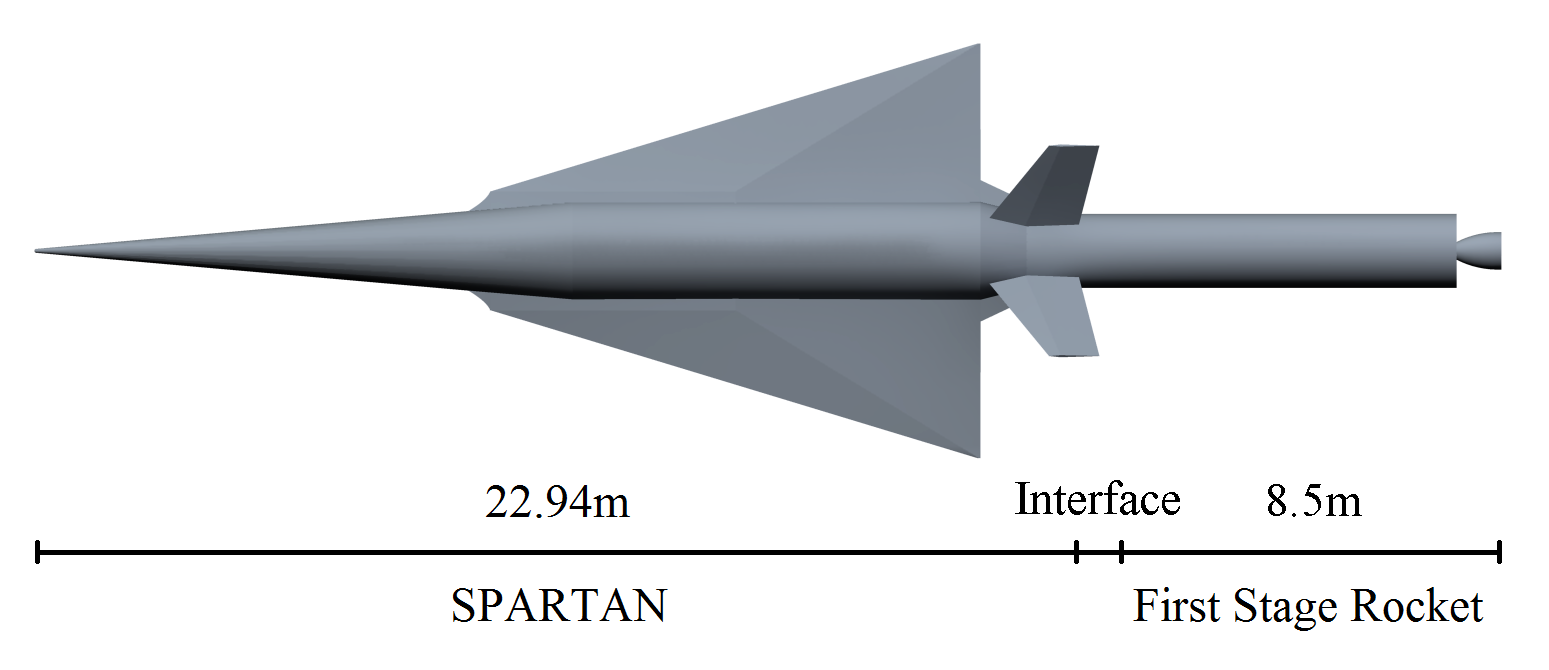
\includegraphics[width=0.7\linewidth]{figures/3_vehicle_design/NoInternal}
\caption{}
\label{fig:NoInternal}
\end{figure}

\begin{figure}
\centering
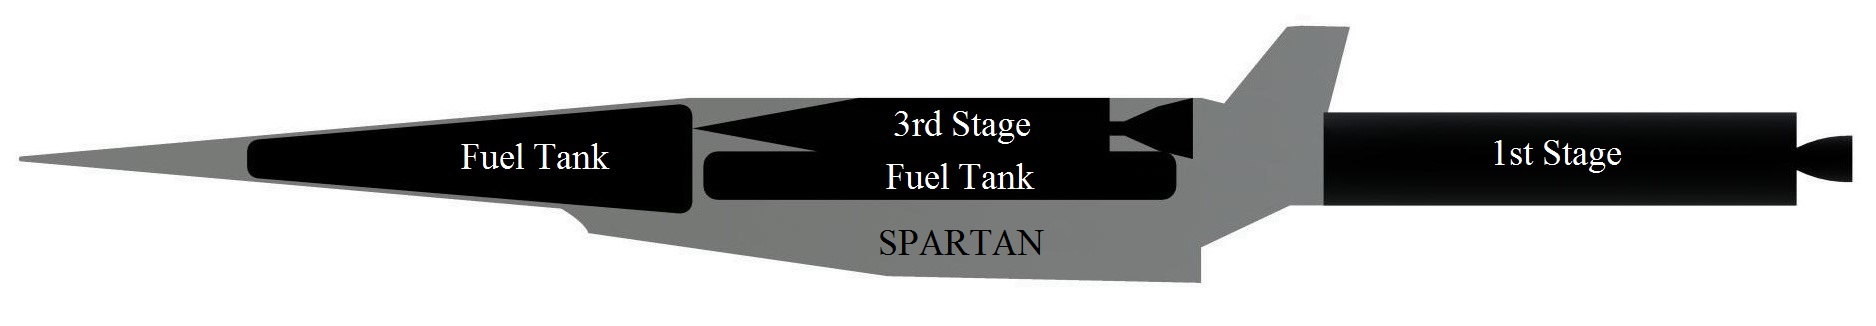
\includegraphics[width=0.7\linewidth]{figures/3_vehicle_design/INTERNALS}
\caption{}
\label{fig:INTERNALS}
\end{figure}


\section{First Stage Rocket}
The first stage rocket-powered vehicle is based on the first stage of the SpaceX Falcon-1e. The Falcon-1e has been chosen due to its appropriate scale, and the proven flightworthiness of the Falcon-1.

	detailed design
	First Stage CART3D
	- details of CAD, pointwise mesh, and CART3D gridding settings
	
	
	\section{Second Stage Scramjet}
		\subsection{Baseline Vehicle}
		The SPARTAN vehicle in this study has been designed based on the work by Preller \& Smart CITATION. 
		
		The baseline SPARTAN has been designed to hold a 9 m long third stage.  Two cylindrical tanks underneath the third stage and a conical tank situated in the nose have a total volume of 22.0m3 and hold a total of 1562kg of LH2 fuel. This assumes an LH2 density of 71kg/m3, slightly denser than LH2 at phase transition point at 1 atm.
		
		 %http://webbook.nist.gov/cgi/fluid.cgi?Action=Load&ID=C1333740&Type=SatT&Digits=5&PLow=.5&PHigh=1.5&PInc=.1&RefState=DEF&TUnit=K&PUnit=atm&DUnit=kg/m3&HUnit=kJ/mol&WUnit=m/s&VisUnit=uPa*s&STUnit=N/m%
		
		
		The fuel tanks are sized to fit around the kestrel-powered third stage, described in Section XX. 
The fuel tanks have a total tank volume of 22.0m$^3$, containing a fuel mass of 1562kg.
The mass of the fuel tanks is scaled from Dawid Prellers model of the SPARTAN, giving a total fuel tank mass of 179.41kg.
		
		
		CG - determined using CREO
		
		\subsection{Aerodynamics}
		method of calculating aerodynamics for trim at required lift
		
		-detail hypaero vs CART3D? 
		
		-detail  CG positioning and shifting during flight as well as method for calculating trim
		
		conical shock calculation
		
		\begin{figure}
\centering
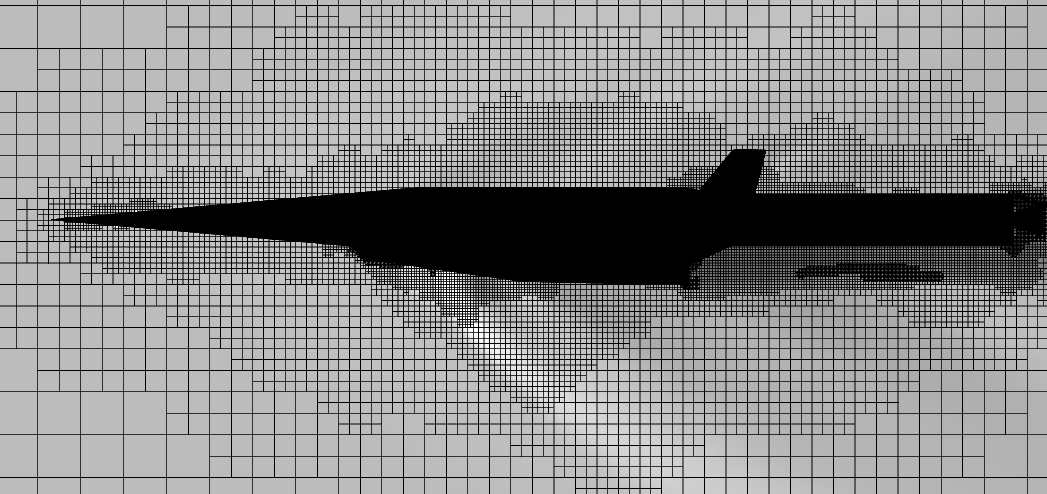
\includegraphics[width=0.7\linewidth]{figures/3_vehicle_design/CARTmesh}
\caption{}
\label{fig:CARTmesh}
\end{figure}
\begin{figure}
\centering
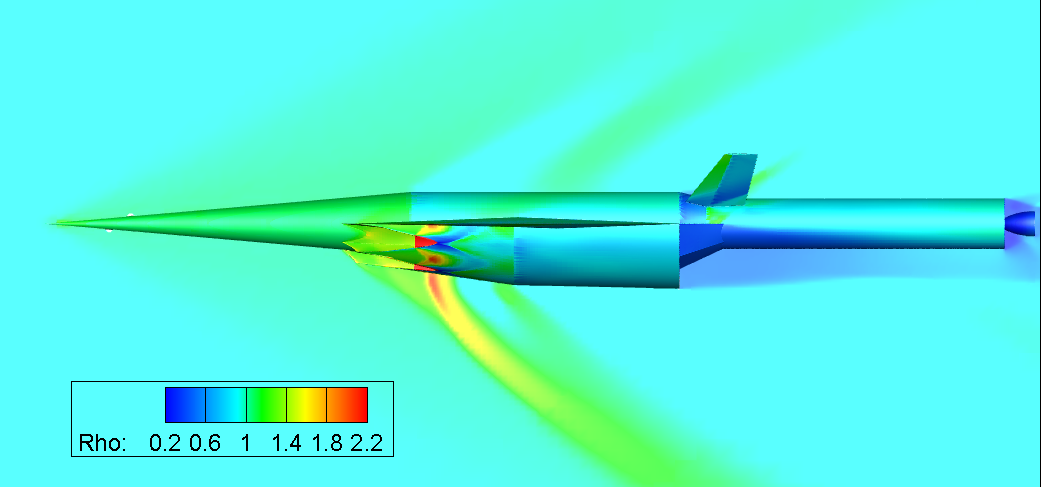
\includegraphics[width=0.7\linewidth]{figures/3_vehicle_design/CARTcontour}
\caption{}
\label{fig:CARTcontour}
\end{figure}


CART3D lift/drag 

Images of CART3D results for a range of Mach numbers



-show side and bottom results for M=0.5,1.1,5,9

\begin{figure}
	\centering
	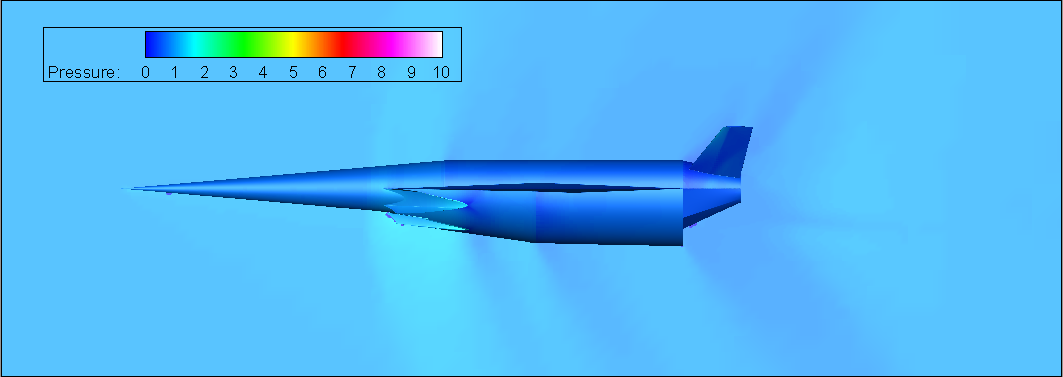
\includegraphics[width=0.7\linewidth]{figures/3_vehicle_design/M1p1AoA6}
	\caption{}
	\label{fig:M1}
\end{figure}
\begin{figure}
	\centering
	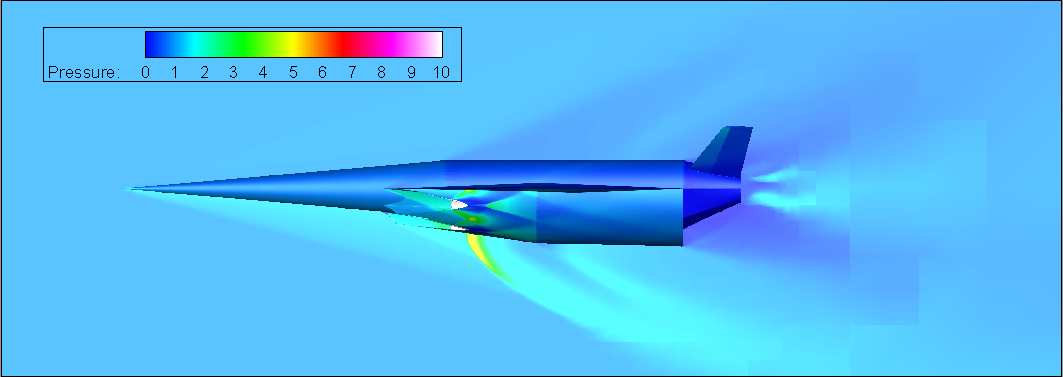
\includegraphics[width=0.7\linewidth]{figures/3_vehicle_design/M3AoA6}
	\caption{}
	\label{fig:M3AoA6}
\end{figure}
\begin{figure}
	\centering
	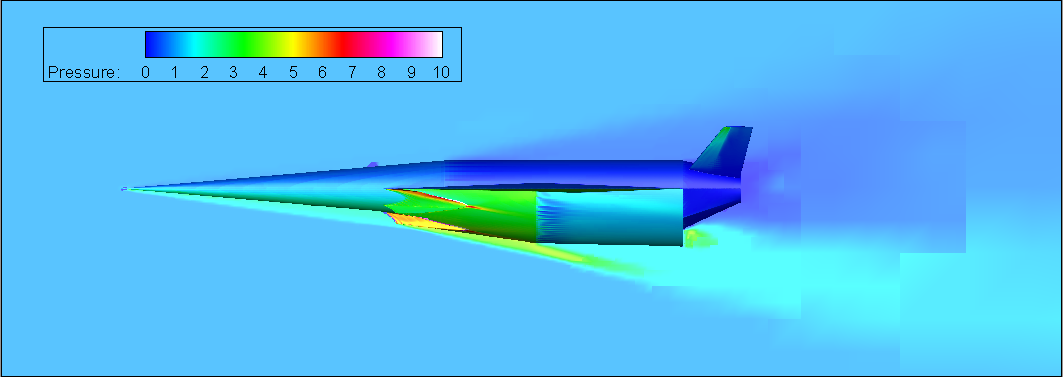
\includegraphics[width=0.7\linewidth]{figures/3_vehicle_design/M7AoA6}
	\caption{}
	\label{fig:M7AoA6}
\end{figure}

\begin{figure}
\centering
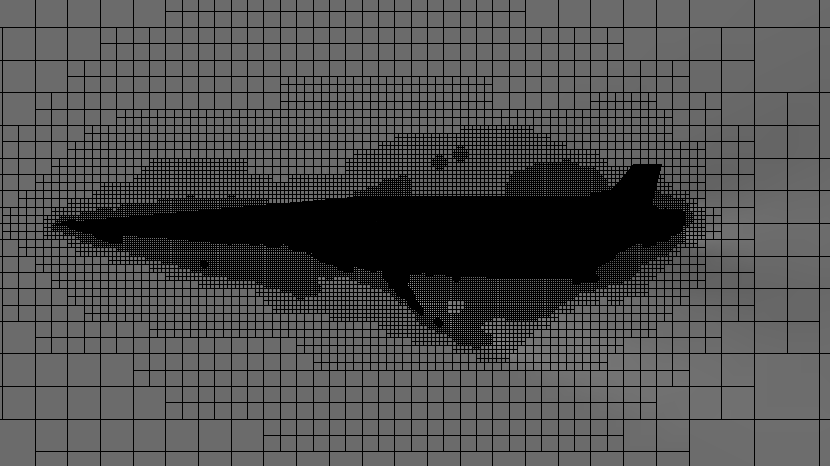
\includegraphics[width=0.7\linewidth]{figures/3_vehicle_design/M3AoA6GRID}
\caption{}
\label{fig:M3AoA6GRID}
\end{figure}


CHANGE THESE GRAPHICS
\begin{figure}
\centering
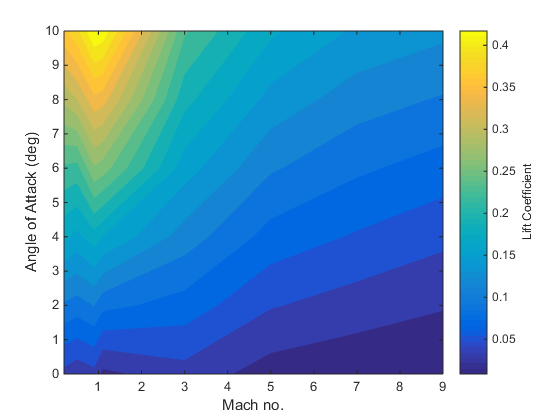
\includegraphics[width=0.7\linewidth]{figures/3_vehicle_design/Cl}
\caption{}
\label{fig:Cl}
\end{figure}
\begin{figure}
\centering
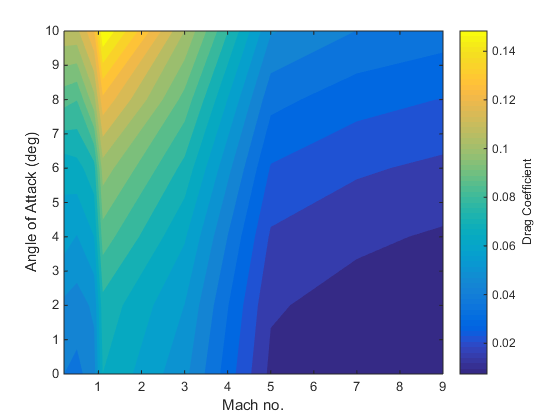
\includegraphics[width=0.7\linewidth]{figures/3_vehicle_design/Cd}
\caption{}
\label{fig:Cd}
\end{figure}
\begin{figure}
\centering
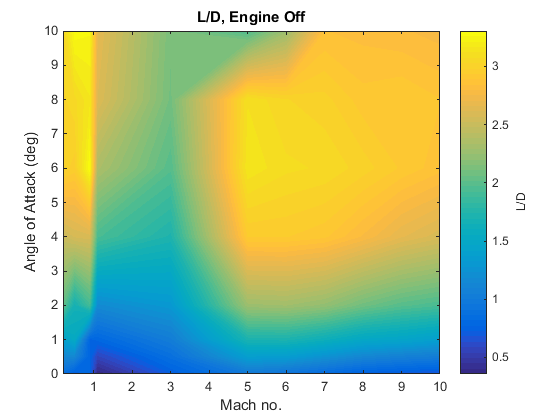
\includegraphics[width=0.7\linewidth]{figures/3_vehicle_design/LD}
\caption{}
\label{fig:LD}
\end{figure}

-put in plots for moments, think about best way to present trim?

\subsection{Engine-On Plume Check}
-simulate engine-on conditions to check that the plumes do not adversely affect the tail of the vehicle (justify that I can just remove engines/boattail)
		
		\subsection{Propulsion Modelling}
		
		\textcolor{red}{conical shock calcs}
		
		\textcolor{red}{C-REST thrust calculator method?}
		
		The SPARTAN is powered by four underslung scramjet engines. These engines are Rectangular To Elliptical Shape Transition (REST) engines, configured to allow for a conical forebody (C-REST). The engine model used is a CRESTM10 database\cite{Preller2017}, analysed using quasi-1D simulation.
	This database provides data points of engine performance over inlet conditions within the operational range, at 50kPa dynamic pressure equivalent conditions. The specific impulse and equivalence ratio data sets are shown in Figure XXX. This data is interpolated for the given inlet conditions to calculate the exit conditions and the specific impulse produced by the engine. The specific impulse is obtained by spline interpolation. As the available dataset is non-uniform in all directions, a linear interpolation is first performed to create a structured grid at all $T_1$ and $M_1$ data point locations. A spline is then fitted to this linearly interpolated grid. The thrust, $T$, is then obtained by inclusion of the mass flow rate ($\dot{m}$) obtained via the inlet conditions, ie. $T = g_0\dot{m}I_{sp}$.
	The C-REST engine is a fixed geometry engine, designed for operability at high Mach numbers\cite{Preller2017}. At lower Mach numbers, the addition of excessive fuel may cause the engine to choke and unstart, resulting in total loss of thrust\cite{Preller2017}. To avoid unstart, an equivalence ratio ($\phi$) of less than 1 is set at low Mach numbers. As the equivalence ratio is equal to 1 in the majority of the Mach number and temperature regime, only the regions in which it is less than 1 are used for the interpolation. The equivalence ratio interpolation is linear, as the number of data points available for interpolation is low. 
	
	
	
	\begin{figure}
\centering
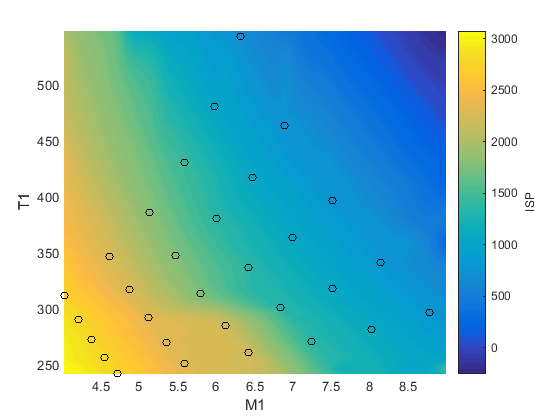
\includegraphics[width=0.7\linewidth]{figures/3_vehicle_design/ISPinterp}
\caption{}
\label{fig:ISPinterp}
\end{figure}

	
	\textcolor{red}{Put Plot of eq Here too}
	\section{Third Stage Rocket}
	
	\begin{figure}
\centering
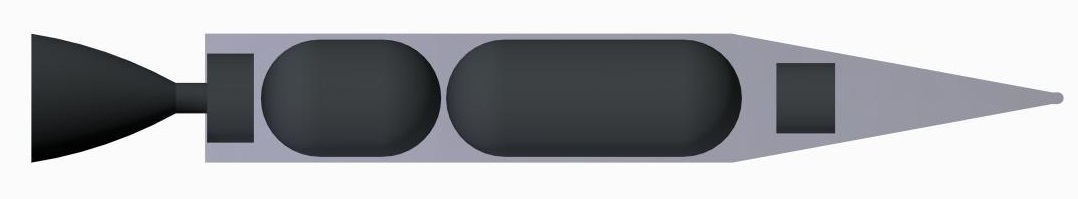
\includegraphics[width=0.7\linewidth]{figures/3_vehicle_design/3rdStage}
\caption{}
\label{fig:3rdStage}
\end{figure}

	The third stage vehicle has been designed to accommodate a SpaceX Kestrel engine. The Kestrel has been chosen for its cost effectiveness and proven capabilities. 
	
	The third stage rocket is released at the end of the scramjet accelerator burn, and lifts the payload out of the atmosphere and into the desired orbit. The third stage weighs a total of 3300kg. The third stage has a structural mass fraction of 0.09, similar to the Falcon 1 second stage \cite{Vehicle2008}. This gives a total structural mass of 285.7kg. 
	
	

	
The kestrel engine has been modified to have 50\% increased propellant mass flow rate, giving a mass flow rate of 14.8kg/s. The nozzle of the Kestrel engine has been kept at XXXm diameter. This increase in mass flow results in a 2\% loss of efficiency from the nozzle\cite{RPE}, due to the thrust coefficient decreasing as shown in Figure \ref{fig:ThrustCoefficient-Arat}. The modified specific impulse of the engine is 310.7s.

	
	Area = 0.866
	
	Lnose = 3m, Centrebody = 4.5m, Engine = 1.5m. Note, some room has been left for the kestrel to go into the body slightly (about 0.5m)
	
	CG - determined using creo, assumed that structure is homogeneous for simplicity
	
	
	\begin{figure}
\centering
\includegraphics[width=0.7\linewidth]{"figures/3_vehicle_design/Thrust Coefficient - Arat"}
\caption{\cite{RPE}}
\label{fig:ThrustCoefficient-Arat}
\end{figure}

		
		\subsection{Fuel Tank Sizing}
		The fuel tanks have been sized assuming 100kg of payload-to-orbit. Note that the method of calculating final payload-to-orbit relies on using left over 'fuel mass' as effective payload mass. Realistically this would cause the fuel tanks to be resized slightly. For the purposes of this study the fuel tanks have been assumed to be of constant size for simplicity. Currently this is a reasonable assumption as the internals of the rocket are very simplified. The structural mass is held constant at 9\%. The third stage carries a total propellant mass of 2736.7kg. Table XX breaks shows the component break-down of the LOX oxidiser and RP1 fuel.  
		
\begin{tabular}{|c|c|c|}
	\hline  & \textbf{LOX} & \textbf{RP1} \\ 
	\hline Ratio & 2.56 & 1 \\ 
	\hline Density & 1141kg/m3 & 813kg/m3 \cite{Magee}\\ 
	\hline Volume & 1.7248m3 & 0.9455m3 \\ 
	\hline Mass & 1968.0 kg & 768.7 kg \\ 
	\hline 
\end{tabular} 
		
		
		
		
		
		
		\subsection{Aerodynamics}
		
		The third stage aerodynamics have been calculated using Missile DATCOM [REFXX], a preliminary design tool for estimating the aerodynamic characteristics of missile and rocket vehicles. Missile DATCOM utilises empirical methods, along with various estimation techniques, to compute the aerodynamics of missile-like vehicles across the subsonic, supersonic and hypersonic regimes.  The code used to compute the aerodynamics of the third stage rocket is detailed in Appendix XX.  
		
		\subsection{Thrust Vectoring}
		
		The third stage rocket is trimmed during the in-atmosphere portion of its ascent trajectory via thrust vectoring. The centre of pressure is calculated using missile DATCOM. The thrust vector is set so that the moment generated by the engine matches the lift force acting at the centre of pressure. The maximum thrust vector limit has been set to 8$^\circ$. As no data on the maximum thrust vectoring capabilities of the kestrel engine was able to be found, this was set to the maximum gimbal range of the Aestus pressure-fed engine and OMS, similar pressure fed engines. 
		
		
		\subsection{Heat Shield Sizing}
		
			The third stage is protected while in-atmosphere by a heat shield, weighting 130.9kg. This heat shield is constructed from a phenolic cork cylinder, a reinforced carbon-carbon nose cone, and a tungsten nose tip. 
		
		
		The tungsten nose is 50mm diameter, at the end of a 50mm Cylinder. The density of tungsten is $\rho_{Tungsten} = 19.25$  g/cm$^3$, giving a total mass for the nose of m = 12.6kg.
		
		Carbon-Carbon shell
		$\rho_{CC} = 1800$  kg/m$^3$
		Thickness of 10mm
		L = 3m
		R = 0.525
		Area = 5.0232m2 ( from Creo)
		
		Anose = 6.22e-2 m2
		
		m = (Area - Anose) t $\rho$ = 89.3kg
		
		
		Cork Cylinder
		t = 5mm
		$\rho_{Cork} = 320$  kg/m$^3$
		
		Area = 14.844m2
		
		m = 23.7kg
		
		
		$m_HS$ = 125.6kg
		